\documentclass{standalone}
\usepackage[]{tikz}
\usetikzlibrary{calc}
\usepackage{ifthen}
\begin{document}
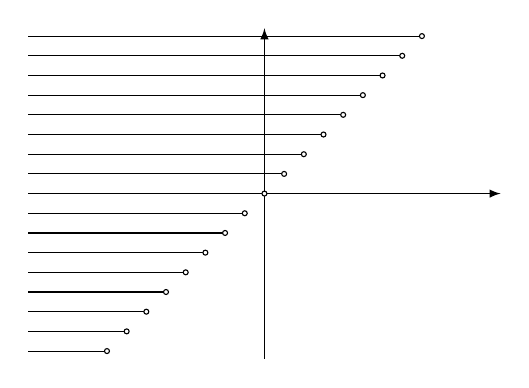
\begin{tikzpicture}
	\draw[-latex] (-3,0) -- (3,0);
	\draw[-latex] (0,-2.1) -- (0,2.1);
	\foreach \i in {-8,...,8}{
		\draw (-3,\i/4) -- (\i/4,\i/4);
		\draw[fill = white] (\i/4,\i/4) circle (.9pt);
	}
\end{tikzpicture}
\end{document}